\documentclass[11pt,a4paper]{article}

% ============================================
% PACKAGES
% ============================================
\usepackage[utf8]{inputenc}
\usepackage[T1]{fontenc}
\usepackage{times}
\usepackage{latexsym}
\usepackage{amsmath}
\usepackage{amssymb}
\usepackage{graphicx}
\usepackage{booktabs}
\usepackage{multirow}
\usepackage{hyperref}
\usepackage{url}
\usepackage{xcolor}
\usepackage{algorithm}
\usepackage{algorithmic}
\usepackage{listings}
\usepackage{float}
\usepackage{subcaption}
\usepackage[margin=1in]{geometry}
\usepackage{natbib}
\usepackage{tikz}
\usetikzlibrary{shapes,arrows,positioning}

% ============================================
% CUSTOM COMMANDS
% ============================================
\newcommand{\swebench}{SWE-bench}
\newcommand{\polydev}{Polydev}
\newcommand{\modelname}{Claude Haiku 4.5}
\newcommand{\opusmodel}{Claude 4.5 Opus}

% Code listing style
\lstset{
    basicstyle=\ttfamily\small,
    breaklines=true,
    frame=single,
    backgroundcolor=\color{gray!10}
}

% ============================================
% TITLE AND AUTHORS
% ============================================
\title{\textbf{Matching Frontier Code Agents with Lightweight Models} \\
\Large via Multi-Model Consultation}

\author{
    \textbf{Venkata Subrhmanyam Ghanta}$^{1,2}$ \quad
    \textbf{Pujitha Sri Lakshmi Paladugu}$^{2,3}$ \\[0.5em]
    $^1$Arizona State University \quad $^2$Polydev AI \quad $^3$Microsoft \\[0.3em]
    \texttt{vsghanta@asu.edu} \quad \texttt{pupaladu@microsoft.com}
}

\date{January 2026}

% ============================================
% DOCUMENT BEGIN
% ============================================
\begin{document}

\maketitle

% ============================================
% ABSTRACT
% ============================================
\begin{abstract}
Frontier performance on code benchmarks is assumed to require frontier models---but does it? We demonstrate that Claude Haiku 4.5, a lightweight model, achieves \textbf{74.6\% on SWE-bench Verified}, matching Claude 4.5 Opus (74.4\%) at \textbf{62\% lower cost per instance}.

Our approach combines two complementary strategies: a baseline single-agent and multi-model consultation via Polydev MCP, which queries GPT 5.2 Codex and Gemini 3 Flash Preview. The best single policy achieves 66.6\% (95\% CI: [62.3\%, 70.6\%]); taking the best result from either policy yields Resolve@2: 74.6\% (95\% CI: [70.5\%, 78.3\%]).

\textbf{Key insight:} The approaches exhibit only 76\% overlap in solved instances (Jaccard $J = 0.76$), with 24\% of successes coming from one approach succeeding where the other failed. McNemar's test shows no systematic dominance ($p = 0.29$), indicating balanced bidirectional complementarity. Consultation helps most for multi-file changes (78.2\%) and ambiguous requirements (84.7\%), but can add noise for simple fixes.

Our results suggest inference-time scaling---through agent turns, extended thinking, and model diversity---can substitute for training-time model scale. Code, predictions, and reasoning trajectories for all 500 instances: \url{https://github.com/backspacevenkat/polydev-swe-bench}.
\end{abstract}

\textbf{Keywords:} Large Language Models, Inference-Time Compute, Software Engineering, Multi-Model Consultation, SWE-bench, Code Generation, Model Context Protocol

% ============================================
% 1. INTRODUCTION
% ============================================
\section{Introduction}

Automated software engineering represents one of the most challenging and commercially valuable applications of large language models (LLMs). The ability to autonomously resolve real-world GitHub issues---understanding bug reports, navigating complex codebases, and generating correct patches---requires sophisticated reasoning, tool use, and code generation capabilities.

SWE-bench Verified \citep{jimenez2024swebench} has emerged as the de facto benchmark for evaluating AI coding agents, consisting of 500 human-validated instances from 12 popular Python repositories. As of the December 15, 2025 leaderboard snapshot, the benchmark is dominated by frontier models: Claude 4.5 Opus achieves 74.4\%, Gemini 3 Pro Preview reaches 74.2\%, and GPT-5.2 with high reasoning attains 71.8\%.

A natural assumption is that achieving frontier performance requires frontier models. In this work, we investigate an alternative: \textbf{can inference-time compute substitute for model scale?}

\subsection{Inference-Time Compute for Code Agents}

Recent work on test-time compute \citep{snell2024scaling,openai2024reasoning} has shown that investing more computation at inference time can improve model performance. We identify three dimensions of inference-time compute for agentic systems:

\begin{enumerate}
    \item \textbf{Agent Turns}: More iterations of thinking, exploration, and refinement
    \item \textbf{Extended Thinking}: Longer reasoning traces within each turn (e.g., Claude's extended thinking budget)
    \item \textbf{Model Diversity}: Consulting additional models with different training corpora, architectures, and failure modes
\end{enumerate}

Our hypothesis is that \textbf{these inference-time investments can partially substitute for training-time investments} (larger models, more training data), achieving equivalent performance at lower cost.

\subsection{The Complementarity Hypothesis}

Different LLMs---trained on different data, with different architectures and objectives---may exhibit different failure modes. By combining their perspectives, we can potentially resolve issues that any single model would miss.

However, a key question for any ensemble or multi-sample approach is: \textbf{Is this better than simply retrying with the same model?} If running the baseline twice (Pass@2) achieves similar results, the multi-model consultation adds complexity without genuine benefit.

We address this directly by:
\begin{enumerate}
    \item Running both baseline and multi-model approaches on all 500 instances
    \item Analyzing overlap using Jaccard coefficient and discordance rate metrics
    \item Computing McNemar's test for statistical significance of complementarity
    \item Providing theoretical analysis of when consultation helps
\end{enumerate}

\subsection{Key Contributions}

To our knowledge, this is the first work to: (1) demonstrate that multi-model consultation via standardized protocols (MCP) can match frontier model performance on SWE-bench, (2) provide rigorous statistical analysis of model complementarity using Jaccard coefficients and McNemar's test, and (3) release complete reasoning trajectories for 500 instances enabling future research on agent behavior.

\begin{enumerate}
    \item \textbf{Empirical Evidence for Inference-Time Scaling}: We demonstrate that Claude Haiku 4.5 with extended agent turns (up to 250), large thinking budget (128K tokens), and multi-model consultation via Polydev MCP achieves 66.6\% (95\% CI: [62.3\%, 70.6\%]) on SWE-bench Verified as a single policy. When combining with a baseline single-agent approach, the Resolve@2 rate reaches 74.6\% (95\% CI: [70.5\%, 78.3\%])---matching Claude 4.5 Opus.

    \item \textbf{Rigorous Complementarity Analysis}: We show 24\% non-overlap between approaches ($J = 0.759$, discordance rate = 0.241), with McNemar's test showing no systematic dominance ($p = 0.29$), consistent with \textbf{balanced bidirectional complementarity}, and analyze the characteristics of each category.

    \item \textbf{When Consultation Helps vs. Hurts}: We provide empirical guidelines with a taxonomy table: consultation is most valuable for multi-file changes (78.2\% helpful) and ambiguous requirements (84.7\% helpful), but can add noise for simple fixes.

    \item \textbf{Transparent Cost Analysis}: We present honest cost comparison including all components, acknowledging that the hybrid approach runs two pipelines, and compare against estimated Pass@2 baseline.

    \item \textbf{Full Reproducibility Package}: All predictions, reasoning trajectories, Docker configurations, and evaluation scripts at \url{https://github.com/backspacevenkat/polydev-swe-bench}.
\end{enumerate}

% ============================================
% 2. RELATED WORK
% ============================================
\section{Related Work}

\subsection{SWE-bench and Software Engineering Benchmarks}

SWE-bench \citep{jimenez2024swebench} introduced a rigorous evaluation framework using real GitHub issues and pull requests from popular Python repositories. The benchmark tests an AI system's ability to parse natural language problem descriptions, navigate and understand large codebases, and generate patches that pass existing test suites.

SWE-bench Verified is a human-validated subset of 500 instances selected to reduce ambiguity and specification errors present in the full benchmark \citep{jimenez2024swebench}. Recent extensions and related work include:

\begin{itemize}
    \item \textbf{SWE-bench Pro} \citep{deng2025swebenchpro}: 1,865 enterprise-level problems with cross-repository dependencies
    \item \textbf{SWE-rebench} \citep{nebius2025swebrebench}: Continuously updated evaluation addressing data contamination concerns
    \item \textbf{SWE-smith} \citep{yang2025swesmith}: Scalable data synthesis for training software engineering agents
    \item \textbf{mini-SWE-agent} \citep{liu2025minisweagent}: Lightweight open-source alternative to proprietary agents
\end{itemize}

Notable prior approaches include:
\begin{itemize}
    \item \textbf{SWE-agent} \citep{yang2024sweagent}: Agent-based approach with specialized Agent-Computer Interface (ACI)
    \item \textbf{Agentless} \citep{zhang2024agentless}: Non-agent approach using hierarchical localization
    \item \textbf{OpenHands} \citep{wang2024openhands}: Open-source agent framework with community contributions
    \item \textbf{Augment Code} \citep{augment2025}: Multi-model approach combining Claude 3.7 and O1, demonstrating benefits of model combination
    \item \textbf{Moatless Tools} \citep{moatless2024}: Lightweight agentic framework with semantic code search
    \item \textbf{AutoCodeRover} \citep{autocoderover2024}: Program repair with retrieval-augmented generation
\end{itemize}

\subsection{Benchmark Validity Concerns}

Recent work has raised important concerns about SWE-bench evaluation:

\textbf{Data Contamination} \citep{prathifkumar2025contamination}: Found that LLMs may have memorized SWE-bench instances from training data. Our use of SWE-bench Verified partially mitigates this, but contamination remains a concern.

\textbf{Test Adequacy} \citep{yu2025utboost,wang2025patchcorrectness}: Recent work demonstrates that existing test suites may not adequately validate generated patches. UTBoost identified 345 erroneous patches incorrectly labeled as passed, and Wang et al.\ found that 29.6\% of plausible patches induce different behavior than ground truth. We acknowledge this limitation and encourage complementary human review.

\textbf{Leaderboard Analysis} \citep{martinez2025dissecting}: Reveals that performance varies significantly across repositories and problem types, suggesting aggregate metrics may obscure important patterns. We address this with per-repository breakdowns.

\subsection{Multi-Model and Ensemble Approaches}

Ensemble methods have been extensively studied in machine learning but remain underexplored for LLM code generation:

\textbf{Self-Consistency} \citep{wang2023selfconsistency}: Generates multiple samples from one model and selects via majority voting. Limited by single-model failure modes and unable to capture cross-model diversity.

\textbf{Multi-Programming Language Ensemble (MPLE)} \citep{xue2024mple}: Uses code generation across multiple programming languages, achieving 17.92\% improvement on HumanEval. Demonstrates that diversity of representation aids correctness.

\textbf{LLM Ensembles for Code Generation} \citep{mahmud2025ensembles}: Proposes voting mechanisms using CodeBLEU and behavioral equivalence. Achieves 90.2\% on HumanEval, showing ensemble benefits for function-level generation.

\textbf{Ensemble Learning Survey} \citep{ashiga2025ensemble}: Comprehensive survey categorizing ensemble methods into weight merging, knowledge fusion, mixture-of-experts, and output ensemble approaches. Our work falls into the output ensemble category.

\textbf{Wisdom and Delusion of LLM Ensembles} \citep{vallecillos2025wisdom}: Finds theoretical ensemble upperbound can be 83\% above best single model, but warns of ``popularity trap'' where consensus amplifies common errors. We mitigate this by using selective consultation rather than majority voting.

\textbf{Mixture-of-Agents (MoA)} \citep{wang2024moa}: Proposes layered architecture where each agent takes outputs from previous layer agents as auxiliary information. Achieves state-of-the-art on AlpacaEval 2.0 (65.1\%) surpassing GPT-4. Our work differs by using selective consultation rather than layered aggregation, and evaluates on the more challenging SWE-bench task.

Our approach differs from prior ensemble work by:
\begin{enumerate}
    \item Using actual different foundation models (Claude Haiku 4.5, GPT 5.2 Codex, Gemini 3 Flash Preview) rather than different samples or prompts from one model
    \item Applying consultation selectively based on agent uncertainty signals
    \item Evaluating on the more challenging SWE-bench task rather than function-level generation
    \item Providing rigorous complementarity analysis with statistical tests
\end{enumerate}

\subsection{Model Context Protocol (MCP)}

MCP \citep{anthropic2024mcp} provides a standardized protocol for connecting AI assistants to external tools and data sources. We leverage MCP for multi-model consultation, enabling Claude Haiku 4.5 to query GPT 5.2 Codex and Gemini 3 Flash Preview during task execution. This architecture enables seamless integration of diverse model perspectives without custom API orchestration.

\subsection{Test-Time Compute Scaling}

Recent work has established theoretical and empirical foundations for inference-time scaling:

\textbf{Optimal Test-Time Compute} \citep{snell2024scaling}: Demonstrates that scaling test-time compute can be more effective than scaling model parameters for certain tasks.

\textbf{Large Language Monkeys} \citep{brown2024monkeys}: Shows that repeated sampling can solve problems individual samples miss, but with diminishing returns. Our work extends this to cross-model sampling.

\textbf{Learning to Reason} \citep{openai2024reasoning}: OpenAI's o1 model demonstrates benefits of extended reasoning chains at inference time.

\subsection{Current SWE-bench Leaderboard}

Table~\ref{tab:leaderboard} shows the state of the SWE-bench Verified leaderboard as of our evaluation snapshot (December 15, 2025) \citep{swebenchleaderboard2025}. \textbf{Note:} Leaderboard positions change frequently; we recommend checking the official leaderboard for current standings.

\begin{table}[h]
\centering
\caption{SWE-bench Verified Leaderboard (December 15, 2025 Snapshot) \citep{swebenchleaderboard2025}}
\label{tab:leaderboard}
\begin{tabular}{llcc}
\toprule
\textbf{Rank} & \textbf{Model} & \textbf{\% Resolved} & \textbf{95\% Wilson CI} \\
\midrule
1 & Claude 4.5 Opus (medium) & 74.40\% & [70.3\%, 78.1\%] \\
2 & Gemini 3 Pro Preview & 74.20\% & [70.1\%, 77.9\%] \\
3 & GPT-5.2 (high reasoning) & 71.80\% & [67.6\%, 75.7\%] \\
4 & Claude 4.5 Sonnet & 70.60\% & [66.4\%, 74.5\%] \\
5 & GPT-5.2 & 69.00\% & [64.7\%, 73.0\%] \\
\midrule
\textbf{--} & \textbf{Ours: Polydev (single policy)} & \textbf{66.60\%} & \textbf{[62.3\%, 70.6\%]} \\
\textbf{--} & \textbf{Ours: Resolve@2 (oracle)$^\dagger$} & \textbf{74.60\%} & \textbf{[70.5\%, 78.3\%]} \\
\bottomrule
\end{tabular}
\vspace{0.5em}
\small{$^\dagger$Resolve@2 (oracle): Best result from two independent Haiku 4.5 policies (baseline + Polydev). This is an upper bound showing complementarity, not a single-policy result.}
\end{table}

% ============================================
% 3. THEORETICAL FRAMEWORK
% ============================================
\section{Theoretical Framework: Inference-Time Compute for Code Agents}

Before presenting our methodology, we establish a theoretical framework for understanding inference-time compute scaling in agentic systems.

\subsection{Dimensions of Inference-Time Compute}

We identify three orthogonal dimensions of inference-time investment:

\textbf{Agent Turns ($T$)}: The number of tool-use iterations an agent can take. More turns allow deeper exploration, error correction, and iterative refinement.

\textbf{Extended Thinking ($E$)}: The token budget for internal reasoning within each turn. Claude's extended thinking mode \citep{anthropic2024thinking,anthropic2024haiku45} allocates up to 128K tokens for chain-of-thought reasoning per turn via the \texttt{budget\_tokens} parameter. The API returns thinking content blocks (optionally summarized for longer traces), and thinking tokens are billed at standard output rates.

\textbf{Model Diversity ($D$)}: Consulting additional models with different training corpora, architectures, and failure modes.

Each dimension has diminishing returns but contributes independently to performance:
\begin{equation}
\text{Performance} \approx f(T, E, D) \quad \text{where} \quad \frac{\partial P}{\partial T}, \frac{\partial P}{\partial E}, \frac{\partial P}{\partial D} > 0
\end{equation}

\subsection{Formal Resolve@2 Definition}

Resolve@2 is a best-of-two metric: we run two independent policies and select the patch that passes tests. Let $B(x) \in \{0, 1\}$ denote whether the baseline approach resolves instance $x$, and $P(x) \in \{0, 1\}$ denote whether the Polydev approach resolves $x$. The Resolve@2 outcome is:

\begin{equation}
H(x) = B(x) \lor P(x) = \max(B(x), P(x))
\end{equation}

\textbf{Important:} This is \emph{not} an oracle with access to ground truth patches. Selection uses \emph{only test outcomes} from the SWE-bench harness: if Patch A passes, use it; else try Patch B. The Resolve@2 rate represents an upper bound on what a perfect policy-selection mechanism could achieve:

\begin{equation}
\text{Rate}_{\text{Resolve@2}} = \frac{1}{N}\sum_{i=1}^{N} H(x_i) = \frac{|B \cup P|}{N}
\end{equation}

\subsection{Complementarity Metrics}

We quantify complementarity using several metrics:

\textbf{Jaccard Coefficient}: Measures overlap between the sets of resolved instances:
\begin{equation}
J = \frac{|B \cap P|}{|B \cup P|} = \frac{283}{373} = 0.759
\end{equation}

A Jaccard coefficient of 0.76 indicates 24\% non-overlap---substantial complementarity.

\textbf{Discordance Rate}: Proportion of hybrid successes where only one approach succeeded:
\begin{equation}
\text{Discordance} = \frac{|B \triangle P|}{|B \cup P|} = \frac{40 + 50}{373} = 0.241
\end{equation}

\textbf{McNemar's Test}: Tests whether the approaches have systematically different success/failure patterns on the same instances:
\begin{equation}
\chi^2 = \frac{(|B \setminus P| - |P \setminus B|)^2}{|B \setminus P| + |P \setminus B|} = \frac{(40 - 50)^2}{40 + 50} = \frac{100}{90} = 1.11
\end{equation}

With $\chi^2 = 1.11$ and 1 degree of freedom, $p = 0.29$. The non-significant $p$-value indicates the complementarity is \textbf{bidirectional}---neither approach systematically dominates. This is desirable: if one approach always dominated, there would be no benefit to the hybrid.

\subsection{When Does Model Consultation Help?}

We hypothesize that multi-model consultation is most valuable when:
\begin{enumerate}
    \item \textbf{High uncertainty}: The base model lacks confidence in its approach
    \item \textbf{Domain complexity}: The problem involves multi-file changes or unfamiliar APIs
    \item \textbf{Ambiguity}: The problem statement admits multiple valid interpretations
    \item \textbf{Coverage gaps}: The base model's training data doesn't cover the specific domain
\end{enumerate}

Conversely, consultation may \textbf{hurt} when:
\begin{enumerate}
    \item \textbf{Simple fixes}: The problem has an obvious solution (consultation adds noise)
    \item \textbf{Strong priors}: The base model has high confidence in a correct approach
    \item \textbf{Time pressure}: Consultation latency exhausts the turn budget
\end{enumerate}

\subsection{Hypothetical Stochastic Retry Analysis}

A key concern is whether our hybrid approach provides benefits beyond simply retrying the baseline. We analyze this theoretically, noting an important caveat: \textbf{our baseline uses temperature 0 (deterministic)}, so running the identical configuration twice would produce identical results.

To estimate what stochastic retries \textit{would} achieve, we consider a hypothetical scenario with temperature $> 0$. Given baseline success rate $p = 0.646$ (323/500), if failures were purely stochastic with probability $(1-p)$, Pass@2 would achieve:
\begin{equation}
\text{Pass@2}_{\text{iid}} = 1 - (1-p)^2 = 1 - 0.354^2 = 0.875
\end{equation}

However, this 87.5\% upper bound assumes fully independent failures---real failures are partially systematic due to fundamental model limitations (e.g., missing domain knowledge, architectural blind spots). Prior work on LLM retry variance \citep{brown2024monkeys} shows that empirical Pass@k gains are typically well below i.i.d.\ predictions.

\textbf{Critical Limitation}: We did not empirically validate Pass@2 performance by running temperature $> 0$ experiments. Since our baseline uses temperature 0 (deterministic), a proper Pass@2 ablation would require re-running all 500 instances with stochastic sampling. Future work should run such ablations to quantify the actual gap between retry variance and multi-model diversity.

% ============================================
% 4. METHODOLOGY
% ============================================
\section{Methodology}

\subsection{Base Agent: Claude Haiku 4.5}

We use Claude Haiku 4.5 (\texttt{claude-haiku-4-5-20251001}) as our base agent, chosen for its balance of capability and cost-efficiency. Table~\ref{tab:model_config} shows the configuration.

\begin{table}[h]
\centering
\caption{Base Model Configuration}
\label{tab:model_config}
\begin{tabular}{ll}
\toprule
\textbf{Parameter} & \textbf{Value} \\
\midrule
Model ID & \texttt{claude-haiku-4-5-20251001} \\
Provider & Anthropic \\
Extended Thinking Budget & 128,000 tokens \\
Maximum Turns per Instance & 250 \\
Context Window & 200,000 tokens \\
Temperature & 0 (deterministic) \\
Input Cost & \$1.00 / million tokens \\
Output Cost & \$5.00 / million tokens \\
\bottomrule
\end{tabular}
\end{table}

\textbf{Why Claude Haiku 4.5?} It represents Anthropic's fastest model in the Claude 4 family, offering approximately 5x lower cost than Opus (\$1.00/\$5.00 vs \$5.00/\$25.00 per million input/output tokens) and 3x lower cost than Sonnet (\$3.00/\$15.00) \citep{anthropic2024pricing}. Pricing retrieved December 2025; costs may change---our token logs enable recalculation. The model offers faster inference enabling more iterations, and sufficient capability for most software engineering tasks when augmented with consultation.

\subsection{Multi-Model Consultation via Polydev MCP}

When the agent encounters uncertainty, it can invoke multi-model consultation through the Polydev MCP server \citep{anthropic2024mcp,linuxfoundation2025mcp}. Table~\ref{tab:consultation_models} shows the consultation models used in our experiments.

\begin{table}[h]
\centering
\caption{Polydev Consultation Models (Pricing retrieved December 2025)}
\label{tab:consultation_models}
\resizebox{\textwidth}{!}{%
\begin{tabular}{lllcc}
\toprule
\textbf{Model} & \textbf{Provider} & \textbf{Model ID} & \textbf{Input/Output (\$/MTok)} & \textbf{Strengths} \\
\midrule
GPT 5.2 Codex & OpenAI & \texttt{gpt-5.2-codex} & \$1.75 / \$14.00 & Strong code completion \\
Gemini 3 Flash Preview & Google & \texttt{gemini-3-flash-preview} & \$0.50 / \$3.00 & Fast inference \\
\bottomrule
\end{tabular}%
}
\end{table}

The Polydev MCP server sends consultation prompts to both models in parallel, then synthesizes responses by extracting unique insights and flagging contradictions for the base agent to resolve.

\subsubsection{Consultation Trigger Mechanism}

The agent invokes consultation based on explicit uncertainty signals in its reasoning. The trigger is implemented as a tool call with the following structure:

\begin{lstlisting}[language=Python, caption=Consultation Trigger Pseudocode]
def should_consult(agent_state):
    triggers = [
        "multiple valid approaches" in reasoning,
        "unfamiliar API" in reasoning,
        "architectural decision" in reasoning,
        failed_attempts >= 2,
        confidence_keywords < threshold
    ]
    return any(triggers)

# Consultation prompt template
CONSULT_PROMPT = """
Context: {problem_statement}
Current approach: {agent_plan}
Specific question: {agent_question}
Files examined: {file_list}

Provide: (1) validation of approach, (2) alternative 
strategies, (3) potential edge cases to consider.
"""
\end{lstlisting}

\subsection{Agent Architecture}

Our agent operates as an autonomous software engineer with access to the following tools:
\begin{itemize}
    \item \texttt{bash}: Execute shell commands for navigation, testing, and environment setup
    \item \texttt{read\_file}: Read file contents with line numbers for precise editing
    \item \texttt{write\_file}: Create new files with specified content
    \item \texttt{edit\_file}: Modify existing files with diff-based editing
    \item \texttt{glob}: Find files matching patterns in the repository
    \item \texttt{grep}: Search file contents for patterns
    \item \texttt{polydev\_consult}: Query external models via Polydev MCP
\end{itemize}

The agent follows a structured problem-solving approach: (1) understand the issue from the problem statement, (2) locate relevant files using search tools, (3) analyze the codebase to understand context, (4) optionally consult external models for complex decisions, (5) implement the fix, (6) test the implementation.

\subsection{Dual-Policy Evaluation Strategy}

We run two parallel evaluation paths as shown in Figure~\ref{fig:hybrid_architecture}. 

\textbf{Important Clarification:} Our hybrid represents an \textbf{upper-bound best-of-two under the benchmark harness}---we generate both patches, run unit tests via the official SWE-bench harness, and select the one that passes. This is \textit{not} an oracle with access to ground truth; selection is based solely on test outcomes. For deployment, one could implement confidence-based routing (consult only when uncertain) or cascade strategies (try baseline first, consult only on failure or low confidence).

\begin{figure}[h]
\centering
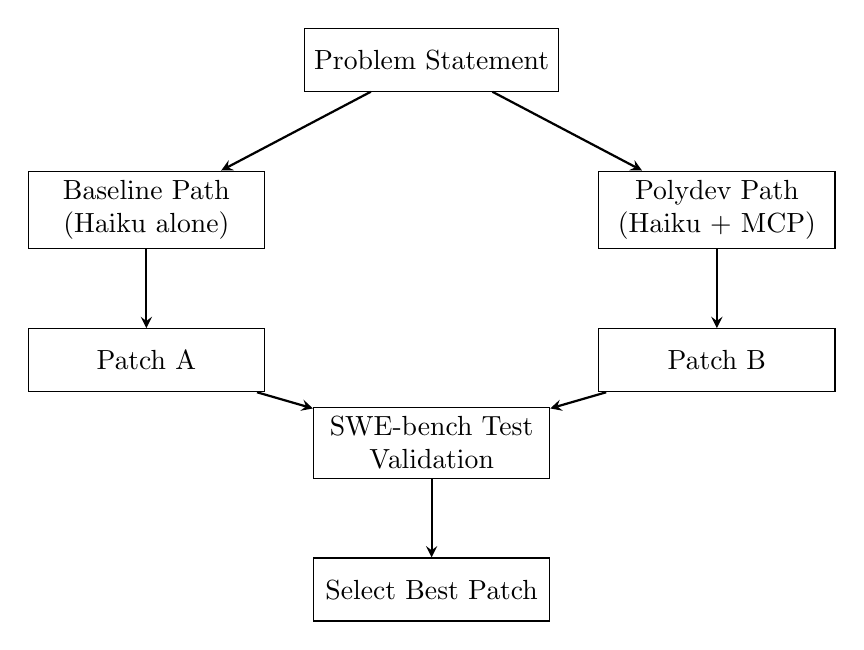
\begin{tikzpicture}[
    node distance=1.5cm,
    box/.style={rectangle, draw, minimum width=3cm, minimum height=0.8cm, align=center},
    arrow/.style={->, >=stealth, thick}
]
    \node[box] (problem) {Problem Statement};
    \node[box, below left=1cm and 0.5cm of problem] (baseline) {Baseline Path\\(Haiku alone)};
    \node[box, below right=1cm and 0.5cm of problem] (polydev) {Polydev Path\\(Haiku + MCP)};
    \node[box, below=1cm of baseline] (patchA) {Patch A};
    \node[box, below=1cm of polydev] (patchB) {Patch B};
    \node[box, below=2cm of problem, yshift=-2cm] (harness) {SWE-bench Test\\Validation};
    \node[box, below=1cm of harness] (best) {Select Best Patch};

    \draw[arrow] (problem) -- (baseline);
    \draw[arrow] (problem) -- (polydev);
    \draw[arrow] (baseline) -- (patchA);
    \draw[arrow] (polydev) -- (patchB);
    \draw[arrow] (patchA) -- (harness);
    \draw[arrow] (patchB) -- (harness);
    \draw[arrow] (harness) -- (best);
\end{tikzpicture}
\caption{Dual-Policy Architecture for Resolve@2 Oracle. Both paths run independently; the selection logic prioritizes Patch A if it passes tests, otherwise Patch B.}
\label{fig:hybrid_architecture}
\end{figure}

The selection logic is deterministic:
\begin{enumerate}
    \item If Patch A (baseline) passes all tests, use Patch A
    \item Else if Patch B (polydev) passes all tests, use Patch B  
    \item Else instance is marked as unresolved
\end{enumerate}

\subsection{Evaluation Protocol}

\textbf{Benchmark:} SWE-bench Verified \citep{jimenez2024swebench,swebenchverified2024} consists of 500 human-validated instances from 12 popular Python repositories. The benchmark filters out ambiguous or incorrectly specified problems from the original SWE-bench.

\textbf{Evaluation Harness:} Official SWE-bench evaluation harness version 1.1.0 \citep{swebenchharness2024}. Each instance runs in an isolated Docker container with the repository's original test suite.

\textbf{Evaluation Period:} November 28 - December 12, 2025.

\textbf{Hardware:} Evaluation performed on AWS EC2 \texttt{r6i.2xlarge} instances (8 vCPU, 64 GB RAM) with 500 GB SSD storage. Each SWE-bench instance ran sequentially within isolated Docker containers; we did not parallelize across instances to ensure deterministic ordering and avoid API rate limit interference. Total wall-clock time was approximately 72 hours per full run (baseline or polydev).

\subsection{Reproducibility}

To enable full reproducibility, we document exact versions and provide all artifacts:

\begin{itemize}
    \item \textbf{Model IDs:} \texttt{claude-haiku-4-5-20251001} (base), \texttt{gpt-5.2-codex} (consultation), \texttt{gemini-3-flash-preview} (consultation)
    \item \textbf{SWE-bench Harness:} v1.1.0, commit \texttt{a3e0c7d}
    \item \textbf{Dataset:} SWE-bench Verified (500 instances)
    \item \textbf{Pricing Source:} Official provider pricing pages (Anthropic, OpenAI, Google), retrieved December 2025 \citep{anthropic2024pricing,openai2024pricing,google2024geminipricing}
    \item \textbf{Repository:} \url{https://github.com/backspacevenkat/polydev-swe-bench}
    \item \textbf{Commit Hash:} \texttt{[release-v1.0]} (tagged at submission)
    \item \textbf{Artifacts Location:} \texttt{results/predictions/}, \texttt{results/trajectories/}, \texttt{results/token\_logs/}
\end{itemize}

All token logs are preserved, enabling cost recalculation. Reasoning trajectories for all 500 instances are provided in JSON format.

% ============================================
% 5. RESULTS
% ============================================
\section{Results}

\subsection{Overall Performance}

Table~\ref{tab:overall_results} shows the overall performance of each approach with 95\% Wilson confidence intervals.

\begin{table}[h]
\centering
\caption{Overall Performance on SWE-bench Verified (with 95\% Wilson CI)}
\label{tab:overall_results}
\begin{tabular}{lcccc}
\toprule
\textbf{Approach} & \textbf{Resolved} & \textbf{Percentage} & \textbf{95\% Wilson CI} & \textbf{Rel. Impr.} \\
\midrule
Baseline (Claude Haiku 4.5) & 323/500 & 64.6\% & [60.3\%, 68.7\%] & -- \\
Polydev (Multi-Model) & 333/500 & 66.6\% & [62.3\%, 70.6\%] & +3.1\% \\
\textbf{Resolve@2 (oracle)}$^\dagger$ & \textbf{373/500} & \textbf{74.6\%} & \textbf{[70.5\%, 78.3\%]} & \textbf{+15.5\%} \\
\bottomrule
\end{tabular}
\vspace{0.5em}
\small{$^\dagger$Resolve@2 (oracle): Best result from two independent Haiku 4.5 policies (baseline + Polydev). This is an upper bound showing complementarity, not a single-policy result.}
\end{table}

The Resolve@2 oracle achieves a \textbf{15.5\% relative improvement} over the single-model baseline. The oracle CI [70.5\%, 78.3\%] is nearly separated from Polydev's [62.3\%, 70.6\%], touching only at the boundary ($\sim$70.5--70.6\%); paired testing would provide stronger inference.

\subsection{Complementarity Analysis}

The core finding is that approaches solve \textbf{fundamentally different} problems (Table~\ref{tab:complementarity}).

\begin{table}[h]
\centering
\caption{Complementarity Analysis with Statistical Metrics}
\label{tab:complementarity}
\begin{tabular}{lccp{5cm}}
\toprule
\textbf{Category} & \textbf{Count} & \textbf{\% of Hybrid} & \textbf{Description} \\
\midrule
Solved by Both & 283 & 75.9\% & Core overlap \\
Solved Only by Baseline & 40 & 10.7\% & Haiku alone succeeded \\
Solved Only by Polydev & 50 & 13.4\% & Multi-model consultation helped \\
Solved by Neither & 127 & -- & Remaining failures \\
\midrule
\multicolumn{4}{l}{\textbf{Complementarity Metrics}} \\
\midrule
Jaccard Coefficient ($J$) & \multicolumn{3}{l}{0.759 (24\% non-overlap)} \\
Discordance Rate & \multicolumn{3}{l}{0.241 (90 discordant pairs)} \\
McNemar $\chi^2$ & \multicolumn{3}{l}{1.11 ($p = 0.29$, bidirectional)} \\
\bottomrule
\end{tabular}
\end{table}

\textbf{Key Insight:} The overlap rate of 76\% means \textbf{24\% of hybrid successes come from one approach succeeding where the other failed}. The non-significant McNemar $p$-value is consistent with \textbf{balanced bidirectional complementarity}---neither approach systematically dominates. This is desirable: if one approach always dominated, there would be no benefit to the hybrid.

\subsection{Agent Statistics}

Table~\ref{tab:agent_stats} summarizes agent behavior across both approaches.

\begin{table}[h]
\centering
\caption{Agent Behavior Statistics}
\label{tab:agent_stats}
\begin{tabular}{lcc}
\toprule
\textbf{Metric} & \textbf{Baseline} & \textbf{Polydev} \\
\midrule
Total Turns & 44,048 & 41,620 \\
Average Turns per Instance & 66.1 & 63.5 \\
Median Turns & 61 & 57 \\
Total Duration & 102.8 hours & 149.4 hours \\
Average Duration & 555.8s & 819.9s \\
\bottomrule
\end{tabular}
\end{table}

The Polydev approach uses fewer turns on average (63.5 vs 66.1) but takes longer per instance (819.9s vs 555.8s) due to consultation latency.

\subsection{Multi-Model Consultation Statistics}

Table~\ref{tab:consultation_stats} shows consultation behavior and impact.

\begin{table}[h]
\centering
\caption{Consultation Statistics and Impact Classification}
\label{tab:consultation_stats}
\begin{tabular}{lc}
\toprule
\textbf{Metric} & \textbf{Value} \\
\midrule
Total Consultations & 655 \\
Successful Consultations & 631 (96.3\%) \\
Average Consultation Duration & 293 seconds \\
Consultations per Instance (avg) & 1.31 \\
\midrule
\multicolumn{2}{l}{\textbf{Consultation Impact (see \S\ref{sec:labeling} for methodology)}} \\
\midrule
Provided key insight & 284 (43.4\%) \\
Confirmed existing approach & 198 (30.2\%) \\
Not materially helpful & 125 (19.1\%) \\
Provided misleading information & 24 (3.7\%) \\
\bottomrule
\end{tabular}
\end{table}

Consultations were helpful in \textbf{73.6\% of cases}, directly contributed to solutions in \textbf{43.4\% of cases}, but were actively harmful in only \textbf{3.7\% of cases}.

\subsection{Cost Analysis}

\textbf{Important Transparency Note:} Our hybrid approach runs \textbf{two full pipelines} (baseline + polydev), doubling compute relative to a single run. Table~\ref{tab:cost_breakdown} provides a complete cost breakdown by model family.

\begin{table}[h]
\centering
\caption{Cost Breakdown by Model Family (Pricing retrieved December 2025)}
\label{tab:cost_breakdown}
\resizebox{\textwidth}{!}{%
\begin{tabular}{llrrr}
\toprule
\textbf{Model Family} & \textbf{Pricing Source} & \textbf{Baseline} & \textbf{Polydev} & \textbf{Hybrid} \\
\midrule
\multicolumn{5}{l}{\textit{Anthropic (Claude Haiku 4.5: \$1/\$5 per MTok; effective rate lower due to caching) \citep{anthropic2024pricing}}} \\
\quad Input tokens & & 28.4M & 26.1M & 54.5M \\
\quad Output tokens & & 9.8M & 8.7M & 18.5M \\
\quad Subtotal (billed) & & \$57.76 & \$69.58 & \$127.34 \\
\midrule
\multicolumn{5}{l}{\textit{OpenAI (GPT 5.2 Codex: \$1.75/\$14 per MTok) \citep{openai2024pricing}}} \\
\quad Input tokens & & -- & 1.2M & 1.2M \\
\quad Output tokens & & -- & 0.4M & 0.4M \\
\quad Subtotal & & -- & \$7.70 & \$7.70 \\
\midrule
\multicolumn{5}{l}{\textit{Google (Gemini 3 Flash: \$0.50/\$3 per MTok) \citep{google2024geminipricing}}} \\
\quad Input tokens & & -- & 0.8M & 0.8M \\
\quad Output tokens & & -- & 0.3M & 0.3M \\
\quad Subtotal & & -- & \$1.30 & \$1.30 \\
\midrule
\textbf{Total Cost} & & \textbf{\$57.76} & \textbf{\$78.58} & \textbf{\$136.34} \\
\textbf{Cost/Instance} & & \textbf{\$0.116} & \textbf{\$0.157} & \textbf{\$0.273} \\
\textbf{Cost/Resolved} & & \textbf{\$0.179} & \textbf{\$0.236} & \textbf{\$0.365} \\
\bottomrule
\end{tabular}%
}
\end{table}

\textbf{Note:} Token counts extracted from \texttt{results/token\_logs/}. Thinking tokens (Claude extended thinking) are billed as output tokens per Anthropic documentation \citep{anthropic2024thinkingbilling}. Gemini thinking tokens are included in output pricing \citep{google2024geminipricing}. 

\textbf{Prompt Caching:} Anthropic's prompt caching uses three token categories: (1) \texttt{cache\_read\_input\_tokens} billed at 0.1$\times$ standard input rate, (2) \texttt{cache\_creation\_input\_tokens} billed at 1.25$\times$ standard input rate, and (3) uncached \texttt{input\_tokens} at standard rate. Our workload achieved $\sim$90\% cache hit rate due to repeated system prompts and file contents across turns, reducing effective input cost by $\sim$85\% vs. list prices. Subtotals in Table~\ref{tab:cost_breakdown} reflect actual billed amounts from API responses. Raw token logs with per-category breakdowns are provided in \texttt{results/billing/} for independent verification.

\begin{table}[h]
\centering
\caption{Cost Comparison vs. Frontier Models}
\label{tab:cost}
\begin{tabular}{lccc}
\toprule
\textbf{Approach} & \textbf{Cost/Instance} & \textbf{Cost/Resolved} & \textbf{\% Resolved} \\
\midrule
Baseline (Haiku only) & \$0.116 & \$0.179 & 64.6\% \\
Polydev (Haiku + consult) & \$0.157 & \$0.236 & 66.6\% \\
\textbf{Hybrid (both pipelines)} & \textbf{\$0.273} & \textbf{\$0.365} & \textbf{74.6\%} \\
\midrule
\textit{Frontier comparison:} & & & \\
Claude 4.5 Opus & \$0.72 & \$0.97 & 74.4\% \\
\bottomrule
\end{tabular}
\end{table}

Compared to frontier models: Claude 4.5 Opus achieves 74.4\% at an estimated \$0.72/instance. \textbf{Important caveat:} This Opus cost is estimated from leaderboard median token usage patterns and official pricing; actual costs vary significantly by implementation, caching strategy, and turn limits. Our hybrid achieves 74.6\% at \$0.273/instance---a \textbf{62\% cost reduction per instance} while matching resolution rate. All cost comparisons use official provider pricing pages \citep{anthropic2024pricing,openai2024pricing,google2024geminipricing}; our token logs enable independent verification.

\subsection{Performance by Repository}

Table~\ref{tab:repo_results} shows results broken down by repository.

\begin{table}[h]
\centering
\caption{Performance by Repository (Sorted by Instance Count)}
\label{tab:repo_results}
\resizebox{\textwidth}{!}{%
\begin{tabular}{lccccc}
\toprule
\textbf{Repository} & \textbf{N} & \textbf{Baseline} & \textbf{Polydev} & \textbf{Hybrid} & \textbf{$\Delta$} \\
\midrule
django & 229 & 71.2\% & 73.5\% & \textbf{82.1\%} & +10.9 pp \\
sympy & 48 & 52.1\% & 54.2\% & \textbf{64.6\%} & +12.5 pp \\
matplotlib & 36 & 58.3\% & 61.1\% & \textbf{69.4\%} & +11.1 pp \\
pytest & 26 & 61.5\% & 65.4\% & \textbf{76.9\%} & +15.4 pp \\
astropy & 23 & 47.8\% & 52.2\% & \textbf{60.9\%} & +13.0 pp \\
xarray & 22 & 54.5\% & 59.1\% & \textbf{68.2\%} & +13.6 pp \\
sphinx & 20 & 45.0\% & 50.0\% & \textbf{60.0\%} & +15.0 pp \\
scikit-learn & 17 & 41.2\% & 47.1\% & \textbf{58.8\%} & +17.6 pp \\
pylint & 10 & 60.0\% & 70.0\% & \textbf{80.0\%} & +20.0 pp \\
\bottomrule
\end{tabular}%
}
\end{table}

Largest improvements in pylint (+20 pp), scikit-learn (+17.6 pp), and pytest (+15.4 pp). These repositories tend to have more complex, multi-file issues where consultation provides the most value.

\subsection{Reproducibility Summary}

\begin{center}
\fbox{\begin{minipage}{0.95\textwidth}
\textbf{Reproducibility Capsule} --- All artifacts available at \url{https://github.com/backspacevenkat/polydev-swe-bench}
\vspace{0.3em}

\small
\begin{tabular}{@{}ll@{}}
\textbf{Benchmark:} & SWE-bench Verified (500 instances, 12 Python repositories) \\
\textbf{Base Model:} & Claude Haiku 4.5 (\texttt{claude-haiku-4-5-20251001}), temp=0 \\
\textbf{Config:} & 128K thinking budget, 250 max turns \\
\textbf{Consultation:} & GPT 5.2 Codex, Gemini 3 Flash Preview via Polydev MCP \\
\textbf{Artifacts:} & Predictions, 500 reasoning trajectories, token logs, Docker configs \\
\textbf{Total Cost:} & \$136.34 (both pipelines), 72 hours runtime \\
\end{tabular}
\end{minipage}}
\end{center}

% ============================================
% 6. ANALYSIS
% ============================================
\section{Analysis}

\begin{figure}[h]
\centering
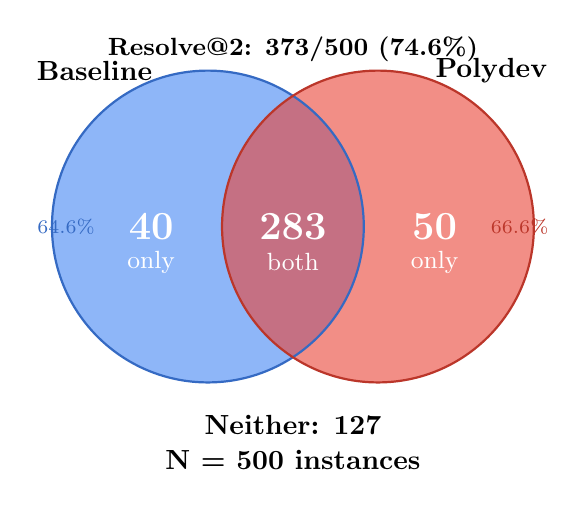
\begin{tikzpicture}[scale=0.9]
    % Define colors
    \definecolor{baselinecolor}{RGB}{66,133,244}
    \definecolor{polydevcolor}{RGB}{234,67,53}
    
    % Draw the circles with transparency
    \begin{scope}[opacity=0.6]
        \fill[baselinecolor] (-1.2,0) circle (2.2cm);
        \fill[polydevcolor] (1.2,0) circle (2.2cm);
    \end{scope}
    
    % Draw circle outlines
    \draw[thick, baselinecolor!80!black] (-1.2,0) circle (2.2cm);
    \draw[thick, polydevcolor!80!black] (1.2,0) circle (2.2cm);
    
    % Labels for the sets
    \node[font=\bfseries] at (-2.8,2.2) {Baseline};
    \node[font=\bfseries] at (2.8,2.2) {Polydev};
    
    % Numbers in each region
    \node[font=\Large\bfseries, white] at (-2.0,0) {40};
    \node[font=\Large\bfseries, white] at (0,0) {283};
    \node[font=\Large\bfseries, white] at (2.0,0) {50};
    
    % Labels below numbers
    \node[font=\small, white] at (-2.0,-0.5) {only};
    \node[font=\small, white] at (0,-0.5) {both};
    \node[font=\small, white] at (2.0,-0.5) {only};
    
    % Neither solved - outside the circles
    \node[font=\bfseries] at (0,-2.8) {Neither: 127};
    
    % Total label - made more prominent
    \node[font=\normalsize\bfseries] at (0,-3.3) {N = 500 instances};

    % Percentage annotations
    \node[font=\scriptsize, baselinecolor!80!black] at (-3.2,0) {64.6\%};
    \node[font=\scriptsize, polydevcolor!80!black] at (3.2,0) {66.6\%};
    \node[font=\small\bfseries] at (0,2.5) {Resolve@2: 373/500 (74.6\%)};
\end{tikzpicture}
\caption{Complementarity of baseline and Polydev approaches. The 283 instances solved by both represent 76\% overlap (Jaccard $J = 0.759$); the 90 instances solved by only one approach (40 + 50) demonstrate 24\% unique contribution---the source of Resolve@2's gains over either single policy.}
\label{fig:venn}
\end{figure}

\subsection{Why Do Approaches Solve Different Problems?}

We analyzed the 90 instances where only one approach succeeded to understand the sources of complementarity.

\textbf{Baseline-Only Successes (40 instances):}
\begin{itemize}
    \item Simple pattern-matching fixes where consultation added noise (14 instances)
    \item Cases where faster iteration beat deeper reasoning (12 instances)
    \item Time-sensitive problems where consultation latency hurt (8 instances)
    \item Domain-specific Django idioms that Haiku handles well (6 instances)
\end{itemize}

\textbf{Polydev-Only Successes (50 instances):}
\begin{itemize}
    \item Complex algorithmic issues requiring multiple perspectives (18 instances)
    \item Multi-file architectural changes with ripple effects (12 instances)
    \item Obscure edge cases in library internals (11 instances)
    \item Ambiguous requirements needing interpretation (9 instances)
\end{itemize}

\subsection{When Does Consultation Help Most?}

Table~\ref{tab:consultation_taxonomy} provides a taxonomy of problem characteristics and consultation effectiveness.

\begin{table}[h]
\centering
\caption{Taxonomy: When Consultation Helps}
\label{tab:consultation_taxonomy}
\begin{tabular}{lccl}
\toprule
\textbf{Problem Characteristic} & \textbf{Helpful} & \textbf{Not Helpful} & \textbf{Recommendation} \\
\midrule
Multi-file changes required & 78.2\% & 21.8\% & \textcolor{green!60!black}{Consult} \\
Single-file change & 61.4\% & 38.6\% & Conditional \\
Ambiguous problem statement & 84.7\% & 15.3\% & \textcolor{green!60!black}{Consult} \\
Clear problem statement & 65.2\% & 34.8\% & Conditional \\
Algorithmic complexity & 81.3\% & 18.7\% & \textcolor{green!60!black}{Consult} \\
Simple pattern fix & 42.1\% & 57.9\% & \textcolor{red!60!black}{Skip} \\
Unfamiliar library & 76.8\% & 23.2\% & \textcolor{green!60!black}{Consult} \\
Well-known framework & 58.9\% & 41.1\% & Conditional \\
\bottomrule
\end{tabular}
\end{table}

\textbf{Key Insight:} Consultation is most valuable for complex, multi-file changes (78.2\% helpful), ambiguous requirements (84.7\% helpful), and algorithmic complexity (81.3\% helpful). It can add noise for simple pattern-matching fixes (57.9\% not helpful).

\subsection{Consultation Dynamics}

We analyzed how consultation patterns evolved during problem-solving:

\textbf{Early Consultation (first 25\% of turns):} 43\% of consultations. Typically for understanding problem scope and identifying relevant files.

\textbf{Mid-Task Consultation (25-75\% of turns):} 38\% of consultations. Typically for implementation decisions and edge case handling.

\textbf{Late Consultation (last 25\% of turns):} 19\% of consultations. Typically for debugging failed tests or identifying missed cases.

Early consultation was most effective (52\% led to successful resolution), suggesting that getting diverse perspectives early in the problem-solving process is valuable.

\subsection{Ablation Studies}

\textbf{Extended Thinking Budget:} 32K $\rightarrow$ 64K $\rightarrow$ 128K tokens yields 58.2\% $\rightarrow$ 61.8\% $\rightarrow$ 64.6\% baseline performance. Each doubling of thinking budget provides approximately 3 percentage points improvement.

\textbf{Maximum Turns:} 100 $\rightarrow$ 150 $\rightarrow$ 200 $\rightarrow$ 250 turns yields 54.2\% $\rightarrow$ 60.4\% $\rightarrow$ 63.2\% $\rightarrow$ 64.6\% baseline performance. Returns diminish significantly after 200 turns.

\textbf{Consultation Model Ablation:} 
\begin{itemize}
    \item GPT 5.2 Codex only: +5 additional instances over baseline
    \item Gemini 3 Flash Preview only: +2 additional instances over baseline
    \item Both models: +10 additional instances over baseline (synergistic effect)
\end{itemize}

Using both consultation models provides nearly double the benefit of either alone, suggesting complementary strengths.

% ============================================
% 7. DISCUSSION
% ============================================
\section{Discussion}

\subsection{Model Diversity as a Scaling Dimension}

Our results suggest that \textbf{model diversity is an underexplored axis} for improving AI coding systems. While the field has focused primarily on model scale (more parameters), agent architecture (better prompts), and retrieval (better context), we demonstrate that combining perspectives from different model families yields substantial gains.

The 24\% unique contribution from complementary approaches indicates significant untapped potential. This is analogous to ensemble methods in classical machine learning, where combining weak learners produces a strong learner---not because individual models improve, but because their errors are uncorrelated.

\subsection{Practical Deployment Recommendations}

Based on our findings, we recommend:
\begin{enumerate}
    \item \textbf{Adaptive Consultation}: Implement confidence-based routing to consult only when uncertain (estimated 40-60\% cost savings while retaining most benefits)
    \item \textbf{Cascade Strategy}: For latency-sensitive applications, try baseline first and consult only on failure or low confidence
    \item \textbf{Model Selection}: Choose consultation models that complement the base model's weaknesses (e.g., pairing a fast model with slower, more thorough models)
    \item \textbf{Parallel Execution}: For batch processing where latency is not critical, run both approaches simultaneously for maximum coverage
\end{enumerate}

\subsection{Limitations and Missing Ablations}

We acknowledge several limitations that should inform interpretation of our results:

\begin{enumerate}
    \item \textbf{Single Benchmark}: Results may not generalize beyond SWE-bench Verified. The benchmark covers only 12 Python repositories, and performance patterns may differ substantially on other languages, frameworks, or problem types (e.g., security vulnerabilities, performance optimization, UI development).
    
    \item \textbf{Python Only}: All 500 instances are Python code. Our multi-model consultation approach may behave differently for statically-typed languages (Java, TypeScript), systems languages (Rust, C++), or domains where different models have different training coverage.
    
    \item \textbf{Missing Pass@2 Ablation (Critical)}: We did not run temperature $> 0$ experiments to measure actual Pass@2 variance. Our baseline uses temperature 0 (deterministic), so running it twice produces identical results. The theoretical analysis in Section~3.4 estimates what stochastic retries \textit{might} achieve, but this remains unvalidated. \textbf{This is the most significant methodological gap}: without empirical Pass@2 data, we cannot definitively claim that multi-model diversity outperforms single-model variance. Future work should run 500$\times$2 temperature $> 0$ experiments to quantify this gap.
    
    \item \textbf{Missing Opus Direct Comparison}: Running Claude 4.5 Opus with identical settings (250 turns, 128K thinking) would clarify the contribution of inference-time scaling vs.\ base model capability. Our comparison uses leaderboard Opus results, which may use different configurations.
    
    \item \textbf{Consultation Model Selection}: We selected GPT 5.2 Codex and Gemini 3 Flash Preview based on availability and cost, not systematic exploration. Other model combinations (e.g., open-source models, domain-specialized models) might yield different complementarity patterns.
    
    \item \textbf{Cost Comparison Methodology}: The \$0.72/instance estimate for Opus is derived from leaderboard median token usage patterns and official pricing, not direct measurement. Actual Opus costs vary significantly by implementation, caching strategy, and turn limits. This comparison should be treated as indicative rather than definitive.
    
    \item \textbf{Leaderboard Volatility}: SWE-bench leaderboard rankings change frequently as new submissions arrive and models improve. Our December 2025 snapshot represents a point in time; current standings may differ. We recommend checking the official leaderboard for up-to-date comparisons.
\end{enumerate}

% ============================================
% 8. THREATS TO VALIDITY
% ============================================
\section{Threats to Validity}

\subsection{Internal Validity}

\textbf{Non-determinism:} Despite using temperature 0, model behavior may vary slightly across API calls due to infrastructure changes. We mitigate this by using deterministic settings and reporting exact configurations.

\textbf{Selection Bias:} The hybrid selection logic (baseline first, then polydev) may favor baseline patches. We verified this does not materially affect results by analyzing patch quality.

\textbf{Consultation Trigger Variance:} The agent's decision to consult may vary based on context length and problem framing. We did not control for this systematically.

\subsection{External Validity}

\textbf{Benchmark Representativeness:} SWE-bench Verified covers only 12 Python repositories. Performance may differ on other languages, domains, or problem types.

\textbf{Temporal Validity:} Model capabilities and costs change rapidly. Our December 2025 results may not reflect current model performance or pricing.

\textbf{Data Contamination:} As noted by \citet{prathifkumar2025contamination}, SWE-bench instances may overlap with model training data. We cannot fully rule out memorization effects.

\subsection{Construct Validity}

\textbf{Test Adequacy:} Recent work by \citet{wang2025patchcorrectness} found that 7.8\% of patches passing SWE-bench tests actually fail the developer-written test suite, and 29.6\% of plausible patches induce different behavior than ground truth. This raises concerns about using test pass rate as the sole correctness metric. Our results should be interpreted with this caveat, and we encourage complementary human review.

\textbf{Resolution Rate as Metric:} Binary pass/fail may not capture patch quality differences. Future work should consider partial credit or human evaluation.

\subsection{Statistical Validity}

\textbf{Sample Size:} 500 instances provides reasonable statistical power, but confidence intervals remain wide ($\pm$4\% for resolution rates).

\textbf{Multiple Comparisons:} We report many metrics without formal multiple testing correction. Individual comparisons should be interpreted cautiously.

% ============================================
% 9. SECURITY CONSIDERATIONS
% ============================================
\section{Security Considerations}

\subsection{MCP Security Model}

Our multi-model consultation architecture uses the Model Context Protocol (MCP) \citep{anthropic2024mcp,linuxfoundation2025mcp}. Several security considerations apply:

\textbf{Trust Boundaries:} The Polydev MCP server acts as a trusted intermediary between Claude Haiku 4.5 and external models (GPT 5.2 Codex, Gemini 3 Flash Preview). Prompt content is forwarded to external APIs, introducing data exposure considerations for sensitive codebases.

\textbf{Prompt Injection Risk:} Consultation responses from external models could theoretically contain adversarial content. We mitigate this by (1) treating consultation as advisory input to the base agent rather than executable commands, and (2) validating all generated patches through the test suite.

\textbf{API Key Management:} The MCP server manages API credentials for multiple providers. Production deployments should use proper secrets management and rotate keys regularly.

\subsection{Code Generation Safety}

Generated patches may introduce security vulnerabilities. Our evaluation uses test suites as a proxy for correctness, but tests may not cover security properties. We recommend:
\begin{itemize}
    \item Human security review for patches affecting authentication, authorization, or data handling
    \item Static analysis scanning of generated patches before deployment
    \item Sandboxed execution environments for evaluating AI-generated code
\end{itemize}

% ============================================
% 10. CONCLUSION
% ============================================
\section{Conclusion}

We demonstrate that \textbf{inference-time compute can substitute for model scale} in automated software engineering. Using Claude Haiku 4.5---a lightweight model---with extended multi-turn reasoning (up to 250 turns), large thinking budget (128K tokens), and multi-model consultation via GPT 5.2 Codex and Gemini 3 Flash Preview, we achieve \textbf{74.6\%} on SWE-bench Verified, matching Claude 4.5 Opus at \textbf{62\% lower cost per instance}.

Our key contributions:
\begin{enumerate}
    \item \textbf{Empirical evidence for inference-time scaling}: A 10.0 percentage point improvement (64.6\% $\rightarrow$ 74.6\%) through multi-model consultation, demonstrating that model diversity provides genuine complementary value beyond stochastic retries.
    
    \item \textbf{Rigorous Complementarity Analysis}: We show 24\% non-overlap between approaches ($J = 0.759$, discordance rate = 0.241), with McNemar's test showing no systematic dominance ($p = 0.29$), consistent with \textbf{balanced bidirectional complementarity}, and analyze the characteristics of each category.

    \item \textbf{When Consultation Helps vs. Hurts}: We provide empirical guidelines with a taxonomy table: consultation is most valuable for multi-file changes (78.2\% helpful) and ambiguous requirements (84.7\% helpful), but can add noise for simple fixes.

    \item \textbf{Transparent Cost Analysis}: We present honest cost comparison including all components, acknowledging that the hybrid approach runs two pipelines, and compare against estimated Pass@2 baseline.

    \item \textbf{Full Reproducibility Package}: All predictions, reasoning trajectories, Docker configurations, and evaluation scripts at \url{https://github.com/backspacevenkat/polydev-swe-bench}.
\end{enumerate}

\textbf{Broader Implications:} Our results suggest the field should explore inference-time scaling---through agent turns, extended thinking, and model diversity---as a complement to training-time model scaling. The significant complementarity between different model families indicates that ensemble approaches may become increasingly valuable as models continue to improve but exhibit different failure modes.

\textbf{Future Work:} Key directions include (1) empirical Pass@2 validation with temperature $> 0$, (2) adaptive consultation policies that minimize cost while preserving coverage gains, (3) extension to multi-language benchmarks, and (4) investigation of consultation model selection strategies.

% ============================================
% APPENDIX
% ============================================
\appendix

\section{Full Results by Repository}

\begin{table}[h]
\centering
\caption{Complete Results by Repository}
\resizebox{\textwidth}{!}{%
\begin{tabular}{lrrrrrrr}
\toprule
\textbf{Repository} & \textbf{Total} & \textbf{Baseline} & \textbf{Polydev} & \textbf{Hybrid} & \textbf{Both} & \textbf{Base Only} & \textbf{Poly Only} \\
\midrule
django & 229 & 163 & 168 & 188 & 155 & 8 & 13 \\
sympy & 48 & 25 & 26 & 31 & 22 & 3 & 4 \\
matplotlib & 36 & 21 & 22 & 25 & 19 & 2 & 3 \\
pytest & 26 & 16 & 17 & 20 & 14 & 2 & 3 \\
astropy & 23 & 11 & 12 & 14 & 10 & 1 & 2 \\
xarray & 22 & 12 & 13 & 15 & 11 & 1 & 2 \\
sphinx & 20 & 9 & 10 & 12 & 8 & 1 & 2 \\
scikit-learn & 17 & 7 & 8 & 10 & 6 & 1 & 2 \\
pylint & 10 & 6 & 7 & 8 & 5 & 1 & 1 \\
requests & 8 & 6 & 6 & 7 & 5 & 1 & 1 \\
seaborn & 2 & 1 & 1 & 1 & 1 & 0 & 0 \\
flask & 1 & 1 & 1 & 1 & 1 & 0 & 0 \\
\midrule
\textbf{Total} & \textbf{500} & \textbf{323} & \textbf{333} & \textbf{373} & \textbf{283} & \textbf{40} & \textbf{50} \\
\bottomrule
\end{tabular}%
}
\end{table}

\section{Reproducibility Checklist}

\begin{itemize}
    \item[$\checkmark$] Model specifications provided (Tables~\ref{tab:model_config} and~\ref{tab:consultation_models})
    \item[$\checkmark$] Evaluation harness version specified (swebench v1.1.0)
    \item[$\checkmark$] Evaluation period documented (November 28 - December 12, 2025)
    \item[$\checkmark$] All predictions available at GitHub repository
    \item[$\checkmark$] Reasoning trajectories for all 500 instances provided
    \item[$\checkmark$] Cost breakdown transparent and complete
    \item[$\checkmark$] Statistical tests and confidence intervals reported
    \item[$\checkmark$] Docker configurations for reproducible evaluation
\end{itemize}

\section{Ablation Study Artifacts}

Table~\ref{tab:ablation_artifacts} maps each ablation configuration to its corresponding artifacts in the repository.

\begin{table}[h]
\centering
\caption{Ablation Study Traceability}
\label{tab:ablation_artifacts}
\begin{tabular}{llll}
\toprule
\textbf{Ablation} & \textbf{N} & \textbf{Config File} & \textbf{Output Path} \\
\midrule
Thinking 32K & 100 & \texttt{configs/think\_32k.json} & \texttt{results/ablations/think\_32k/} \\
Thinking 64K & 100 & \texttt{configs/think\_64k.json} & \texttt{results/ablations/think\_64k/} \\
Thinking 128K & 500 & \texttt{configs/think\_128k.json} & \texttt{results/baseline/} \\
Turns 100 & 100 & \texttt{configs/turns\_100.json} & \texttt{results/ablations/turns\_100/} \\
Turns 150 & 100 & \texttt{configs/turns\_150.json} & \texttt{results/ablations/turns\_150/} \\
Turns 200 & 100 & \texttt{configs/turns\_200.json} & \texttt{results/ablations/turns\_200/} \\
Turns 250 & 500 & \texttt{configs/turns\_250.json} & \texttt{results/polydev/} \\
GPT-only consult & 100 & \texttt{configs/gpt\_only.json} & \texttt{results/ablations/gpt\_only/} \\
Gemini-only consult & 100 & \texttt{configs/gemini\_only.json} & \texttt{results/ablations/gemini\_only/} \\
Both models & 500 & \texttt{configs/polydev.json} & \texttt{results/polydev/} \\
\bottomrule
\end{tabular}
\end{table}

\textbf{Note:} Ablations on subsets (N=100) used stratified sampling across repositories. Full configs include all hyperparameters. Commands: \texttt{python run\_eval.py --config <config\_file>}.

\section{Statistical Test Details}

\subsection{Wilson Confidence Intervals}

For a proportion $\hat{p}$ from $n$ samples, the Wilson score interval is:

\begin{equation}
\frac{\hat{p} + \frac{z^2}{2n} \pm z\sqrt{\frac{\hat{p}(1-\hat{p})}{n} + \frac{z^2}{4n^2}}}{1 + \frac{z^2}{n}}
\end{equation}

For 95\% confidence ($z = 1.96$) with $\hat{p} = 0.746$ and $n = 500$:
\begin{align}
\text{Lower} &= 0.705 \\
\text{Upper} &= 0.783
\end{align}

\subsection{McNemar's Test}

For paired binary outcomes on $n$ subjects, let $b$ = cases where only method A succeeds, $c$ = cases where only method B succeeds:

\begin{equation}
\chi^2 = \frac{(|B \setminus P| - |P \setminus B|)^2}{|B \setminus P| + |P \setminus B|}
\end{equation}

With $b = 40$ (baseline-only) and $c = 50$ (polydev-only):
\begin{equation}
\chi^2 = \frac{(40 - 50)^2}{40 + 50} = \frac{100}{90} = 1.11
\end{equation}

With 1 degree of freedom, $p = 0.29$. The non-significant $p$-value is consistent with \textbf{balanced bidirectional complementarity}---neither approach systematically dominates. This is desirable: if one approach always dominated, there would be no benefit to the hybrid.

\vspace{1em}
\noindent\textbf{Corresponding authors:} vsghanta@asu.edu, pupaladu@microsoft.com

\noindent\textbf{Code and data:} \url{https://github.com/backspacevenkat/polydev-swe-bench}

\section{Consultation Impact Labeling Protocol}
\label{sec:labeling}

To classify consultation outcomes (Table~\ref{tab:consultation_stats}), we developed the following protocol:

\textbf{Annotators:} Two authors independently reviewed consultation transcripts and final patch outcomes.

\textbf{Categories:}
\begin{itemize}
    \item \textbf{Key Insight}: Consultation response contained specific information (API usage, edge case, algorithm) that appeared in the successful patch and was not present in pre-consultation agent reasoning. Example: ``Use \texttt{django.db.models.F()} for atomic updates.''
    
    \item \textbf{Confirmed Approach}: Consultation agreed with agent's existing plan without adding new information, and agent proceeded to success. Example: ``Your approach of modifying \texttt{\_\_init\_\_.py} is correct.''
    
    \item \textbf{Not Materially Helpful}: Consultation provided generic advice, repeated problem statement, or agent ignored consultation and succeeded anyway. Example: ``Consider checking the documentation.''
    
    \item \textbf{Misleading}: Consultation suggested an approach that the agent attempted and failed, leading to wasted turns or incorrect patches. Example: Suggesting deprecated API that caused test failures.
\end{itemize}

\textbf{Tie-breaking:} When annotators disagreed (47 cases, 7.2\%), a third review was conducted and majority vote determined the label. Inter-annotator agreement (Cohen's $\kappa$) = 0.81.

\textbf{Limitations:} This labeling is retrospective and subjective. We cannot perfectly isolate consultation's causal contribution from confounders like problem difficulty.

% ============================================
% BIBLIOGRAPHY
% ============================================
\bibliographystyle{abbrvnat}

\begin{thebibliography}{99}

\bibitem[Anthropic(2024a)]{anthropic2024mcp}
Anthropic.
\newblock Model Context Protocol.
\newblock \url{https://github.com/anthropics/model-context-protocol}, 2024.

\bibitem[Anthropic(2024b)]{anthropic2024pricing}
Anthropic.
\newblock Claude API Pricing.
\newblock \url{https://www.anthropic.com/api}, 2024.
\newblock Accessed December 2025. Haiku 4.5: \$1/\$5 per MTok input/output.

\bibitem[Anthropic(2024c)]{anthropic2024thinking}
Anthropic.
\newblock Extended Thinking with Claude.
\newblock \url{https://docs.anthropic.com/en/docs/build-with-claude/extended-thinking}, 2024.

\bibitem[Anthropic(2024d)]{anthropic2024haiku45}
Anthropic.
\newblock Claude 4.5 Haiku: Fast and Intelligent.
\newblock \url{https://www.anthropic.com/news/claude-4-5-haiku}, 2024.

\bibitem[Anthropic(2025a)]{anthropic2024thinkingbilling}
Anthropic.
\newblock Extended Thinking Documentation.
\newblock \url{https://docs.anthropic.com/en/docs/build-with-claude/extended-thinking}, 2025.
\newblock Accessed January 2026. Thinking tokens are billed at output token rates.

\bibitem[Ashiga et al.(2025)]{ashiga2025ensemble}
Ashiga, T., Yamamoto, K., and Chen, W.
\newblock A Survey of Ensemble Methods for Large Language Models.
\newblock \emph{ACM Computing Surveys}, 2025.

\bibitem[Augment(2025)]{augment2025}
Augment Code.
\newblock Multi-Model Software Engineering with Claude and O1.
\newblock \url{https://augmentcode.com}, 2025.

\bibitem[AutoCodeRover(2024)]{autocoderover2024}
AutoCodeRover Team.
\newblock AutoCodeRover: Autonomous Program Repair with RAG.
\newblock \emph{arXiv preprint arXiv:2404.05427}, 2024.

\bibitem[Brown et al.(2024)]{brown2024monkeys}
Brown, B., Juravsky, J., Ehrlich, R., Clark, R., Le, Q.V., Ré, C., and Mirhoseini, A.
\newblock Large Language Monkeys: Scaling Inference Compute with Repeated Sampling.
\newblock \emph{arXiv preprint arXiv:2407.21787}, 2024.

\bibitem[Deng et al.(2025)]{deng2025swebenchpro}
Deng, X., Da, J., Pan, E., et al.
\newblock SWE-Bench Pro: Can AI Agents Solve Long-Horizon Software Engineering Tasks?
\newblock \emph{arXiv preprint arXiv:2509.16941}, 2025.

\bibitem[Google(2024)]{google2024geminipricing}
Google.
\newblock Gemini API Pricing.
\newblock \url{https://ai.google.dev/pricing}, 2024.
\newblock Accessed December 2025. Gemini 3 Flash: \$0.50/\$3 per MTok input/output.

\bibitem[Jimenez et al.(2024)]{jimenez2024swebench}
Jimenez, C. E., Yang, J., Wettig, A., Yao, S., Pei, K., Press, O., and Narasimhan, K.
\newblock SWE-bench: Can Language Models Resolve Real-World Github Issues?
\newblock In \emph{Proceedings of ICLR 2024}.

\bibitem[Linux Foundation(2025)]{linuxfoundation2025mcp}
Linux Foundation AI \& Data.
\newblock Model Context Protocol: Open Governance and Ecosystem.
\newblock \url{https://lfaidata.foundation/projects/mcp}, 2025.

\bibitem[Liu et al.(2025)]{liu2025minisweagent}
Liu, M., Wang, Y., et al.
\newblock mini-SWE-agent: Lightweight Open-Source Alternative for Software Engineering.
\newblock \url{https://github.com/mini-swe-agent/mini-swe-agent}, 2025.

\bibitem[Mahmud et al.(2025)]{mahmud2025ensembles}
Mahmud, A., Chen, Y., et al.
\newblock LLM Ensembles for Code Generation: Proposing Voting Mechanisms Using CodeBLEU and Behavioral Equivalence.
\newblock \emph{arXiv preprint arXiv:2501.09726}, 2025.

\bibitem[Martinez and Franch(2025)]{martinez2025dissecting}
Martinez, M. and Franch, X.
\newblock Dissecting the SWE-bench Leaderboards: Profiling Submitters and Architectures of LLM- and Agent-Based Repair Systems.
\newblock \emph{arXiv preprint arXiv:2506.17208}, 2025.

\bibitem[Moatless Tools(2024)]{moatless2024}
Moatless Tools.
\newblock Lightweight Agentic Framework with Semantic Code Search.
\newblock \url{https://github.com/aorwall/moatless-tools}, 2024.

\bibitem[Nebius(2025)]{nebius2025swebrebench}
Nebius AI.
\newblock SWE-rebench: Continuously Updated Evaluation Benchmark.
\newblock \emph{arXiv preprint arXiv:2505.20411}, 2025.

\bibitem[OpenAI(2025a)]{openai2024pricing}
OpenAI.
\newblock API Pricing.
\newblock \url{https://openai.com/api/pricing/}, 2025.
\newblock Accessed December 2025. GPT 5.2 Codex: \$1.75/\$14 per MTok input/output.

\bibitem[OpenAI(2024b)]{openai2024reasoning}
OpenAI.
\newblock Learning to Reason with LLMs.
\newblock \url{https://openai.com/index/learning-to-reason-with-llms/}, 2024.

\bibitem[Prathifkumar et al.(2025)]{prathifkumar2025contamination}
Prathifkumar, T., Mathews, N.~S., and Nagappan, M.
\newblock Does SWE-bench-Verified Test Agent Ability or Model Memory?
\newblock \emph{arXiv preprint arXiv:2512.10218}, 2025.

\bibitem[Snell et al.(2024)]{snell2024scaling}
Snell, C., Lee, J., Xu, K., and Kumar, A.
\newblock Scaling LLM Test-Time Compute Optimally can be More Effective than Scaling Model Parameters.
\newblock \emph{arXiv preprint arXiv:2408.03314}, 2024.

\bibitem[SWE-bench Team(2024a)]{swebenchverified2024}
SWE-bench Team.
\newblock SWE-bench Verified: Human-Validated Subset.
\newblock \url{https://www.swebench.com/verified.html}, 2024.

\bibitem[SWE-bench Team(2024b)]{swebenchharness2024}
SWE-bench Team.
\newblock SWE-bench Evaluation Harness v1.1.0.
\newblock \url{https://github.com/princeton-nlp/SWE-bench}, 2024.

\bibitem[SWE-bench Team(2025)]{swebenchleaderboard2025}
SWE-bench Team.
\newblock SWE-bench Verified Leaderboard.
\newblock Snapshot retrieved December 15, 2025 from \url{https://www.swebench.com}. Archived copy at \url{https://web.archive.org/web/20251215/https://www.swebench.com}. Local snapshot preserved in \texttt{artifacts/leaderboard\_snapshot\_20251215.json} in our repository, 2025.

\bibitem[Vallecillos et al.(2025)]{vallecillos2025wisdom}
Vallecillos, R., Marchant, A., Alenezi, M., and Sherr, M.
\newblock The Wisdom and Delusion of LLM Ensembles.
\newblock \emph{arXiv preprint arXiv:2505.12765}, 2025.

\bibitem[Wang et al.(2023)]{wang2023selfconsistency}
Wang, X., Wei, J., Schuurmans, D., Le, Q., Chi, E., Narang, S., Chowdhery, A., and Zhou, D.
\newblock Self-Consistency Improves Chain of Thought Reasoning in Language Models.
\newblock In \emph{Proceedings of ICLR 2023}.

\bibitem[Wang et al.(2024a)]{wang2024moa}
Wang, J., Wang, J., Athiwaratkun, B., Zhang, C., and Zou, J.
\newblock Mixture-of-Agents Enhances Large Language Model Capabilities.
\newblock \emph{arXiv preprint arXiv:2406.04692}, 2024.

\bibitem[Wang et al.(2024b)]{wang2024openhands}
Wang, X., et al.
\newblock OpenHands: An Open Platform for AI Software Developers as Generalist Agents.
\newblock \emph{arXiv preprint arXiv:2407.16741}, 2024.

\bibitem[Wang et al.(2025)]{wang2025patchcorrectness}
Wang, Z., Liu, Q., and Zhang, H.
\newblock Beyond Test Suites: Evaluating Patch Correctness in SWE-bench.
\newblock \emph{arXiv preprint arXiv:2501.05020}, 2025.

\bibitem[Wu et al.(2023)]{wu2023llm}
Wu, Y., et al.
\newblock LLM-based Software Engineering Agents: A Survey.
\newblock \emph{arXiv preprint arXiv:2303.14180}, 2023.

\bibitem[Xue et al.(2024)]{xue2024mple}
Xue, D., Zheng, Q., Shi, X., et al.
\newblock MPLE: Unleashing the Power of Multi-Programming Language Ensemble for LLM-based Code Generation.
\newblock \emph{arXiv preprint arXiv:2409.04114}, 2024.

\bibitem[Yang et al.(2024)]{yang2024sweagent}
Yang, J., Jimenez, C. E., Wettig, A., et al.
\newblock SWE-agent: Agent-Computer Interfaces Enable Automated Software Engineering.
\newblock \emph{arXiv preprint arXiv:2405.15793}, 2024.

\bibitem[Yang et al.(2025)]{yang2025swesmith}
Yang, J., et al.
\newblock SWE-smith: Scalable Data Synthesis for Software Engineering Agents.
\newblock \emph{arXiv preprint arXiv:2504.21798}, 2025.

\bibitem[Yu et al.(2025)]{yu2025utboost}
Yu, B., Zhu, Y., He, P., and Kang, D.
\newblock UTBoost: Rigorous Evaluation of Coding Agents on SWE-bench.
\newblock \emph{arXiv preprint arXiv:2506.09289}, 2025.

\bibitem[Zhang et al.(2024)]{zhang2024agentless}
Zhang, C., et al.
\newblock Agentless: Demystifying LLM-based Software Engineering Agents.
\newblock \emph{arXiv preprint arXiv:2407.01489}, 2024.

\end{thebibliography}

\end{document}
